\documentclass[11pt,a4paper]{article}
\usepackage{od}
\usepackage[utf8]{inputenc}
\usepackage[ngerman]{babel}

\pagestyle{headings}
\title{Cup des TRIZ-Summits – 2019/2020}

\author{Übersetzung des Textes ins Deutsche: Hans-Gert Gr\"abe, Leipzig}

\date{6. November 2019}

\newcommand{\video}{Die Clips sollten kurz sein (2 bis 5 Minuten). Es müsssen
  alle Autoren angegeben werden: Drehbuchautor, Kameramann, Cutter,
  Schauspieler usw.

Diese Arbeit zielt auf die Erstellung von Lehrmaterial für die
TRIZ-Ausbildung.

Auf der Website des TRIZ-Summit\footnote {\url
  {http://triz-summit.ru/en/contest/competition/video/}, \\ \url
  {https://www.youtube.com/channel/UCjMNOjboWRBQA72DJvaC7ew/featured}}
sind Videos vom letzten TRIZ Summit Cup veröffent\-licht.}

\newcommand{\credentials}{Die Aufgaben des TRIZ Summit Cup 2018/2019 wurden
  vorbereitet von Rubin M.S., Rubina N.V., die Nomination „Fantasie“ stammt
  von P.R. Amnuel.}

\newcommand{\melies}{
\begin{minipage}{.6\textwidth}
  \paragraph{1.}
  Der Gründer des Science-Fiction-Genres ist der französische Filmemacher
  Georges Méliès. Jeder der über 500 Kurzfilme, die von Méliès erstellt
  wurden, zeichnet sich durch einen einzigartigen „Regiestil“ aus. Im Film
  „Besuch des Wracks des Kreuzers Maine“ (1897--1898) in der Folge „Taucher
  bei der Arbeit“ war es notwendig, ein klares Bild von Menschen zu zeigen,
  die unter Wasser arbeiten, und auch ein klares Bild von den Trümmern des
  Kreuzers.  Bilder unter Wasser wurden zu jener Zeit bereits aufgenommen,
  aber sie waren eher exotisch und nicht gut genug sogar in sehr klarem
  Wasser. Schauen Sie sich zum Beispiel eines der ersten Fotos unter Wasser
  an, aufgenommen 1893 in Frankreich (Sie sind sicher einverstanden, dass die
  Qualität nicht für eine Filmepisode ausreicht). Wie hat man es geschafft,
  eine Episode unter Wasser in guter Qualität zu drehen? 
\end{minipage} \hfill
\begin{minipage}{.35\textwidth}
  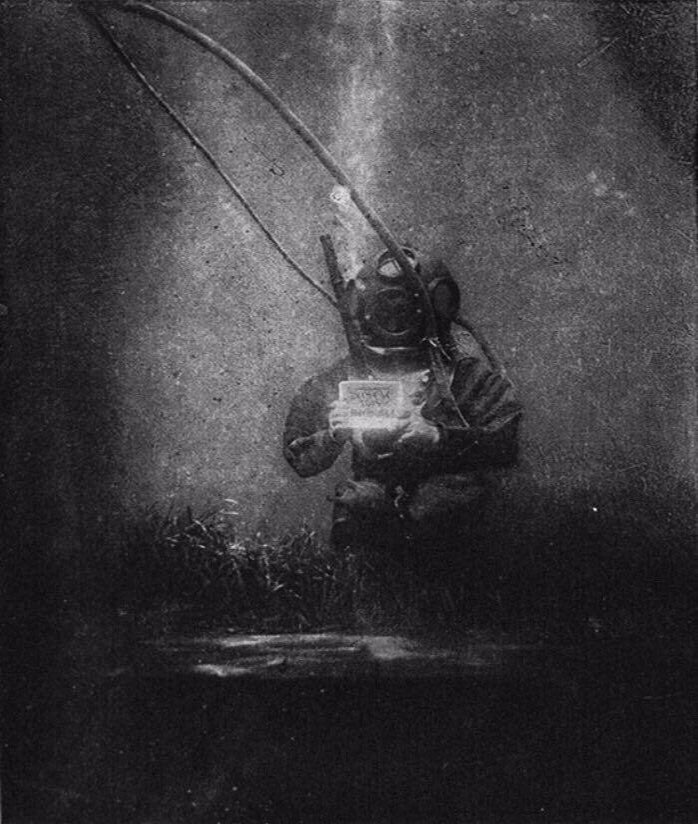
\includegraphics[width =\textwidth]{Bild-1.jpg}
\end{minipage}
\medskip

Der Film von J. Méliès „Im Reich der
Feen“\footnote{\url{https://www.youtube.com/watch?v=paM_BPyRT1o&t=542s}} setzt
ähnliche Wirkungen ein.

Überraschenderweise verwendete Alexander Ptuschko den gleichen Spezialeffekt
im Film\-märchen „Sadko“ im Jahr 1952 in Szenen auf dem Meeresboden in der
Nähe des Meereskönigs.

Welche weiteren Spezialeffekte werden im Kino eingesetzt zur Lösung welcher
Probleme? Welche Widersprüche entstehen dabei und durch welche Methoden werden
sie gelöst?  }

\newcommand{\hollywood}{\paragraph{2.}  In der Geschichte der Schaffung des
  größten Filmkonzerns der Welt -- Hollywood -- gibt es Episoden, die sich
  nicht auf das künstlerische Schaffen oder auf die Erfindung neuer
  technischer Mittel für die Erstellung eines Films beziehen, sondern auf rein
  rechtliche Probleme. Zu Beginn des 20. Jahrhunderts gehörten die
  Hauptpatente für Kinogeräte in Amerika Thomas Edison (der Erfinder, auch der
  Glühlampen). Die meisten Filmemacher dieser Zeit waren jedoch Eigentümer von
  unabhängigen Filmunternehmen. Außerdem arbeiteten sie alle mit Geräten, die
  sie selbst verbessert und an die Umsetzung ihrer Filmideen angepasst hatten.
  Aus diesen Gründen hielten sie es nicht für notwendig, Edison Prozente für
  die Nutzung seiner Patente zu bezahlen. Am 18. Dezember 1908 gab Edison die
  Gründung der Motion Picture Patents Company (MPPC) bekannt, die in die
  Geschichte des Kinos eingegangen ist wie der Edison Trust. Einige Filmfirmen
  haben sich dem Trust angeschlossen, die meisten jedoch blieben unabhängig.
  Der 24. Dezember 1908, als die Gründung des Trusts juristisch wirksam wurde,
  wurde in der Geschichte des amerikanischen Kinos berühmt als „schwarze
  Weihnachten“. Nach Edisons Regeln mussten die unabhängigen Filmfirmen dem
  Trust enorme Summen für das Recht zahlen, Filme aufzunehmen und Filme zu
  zeigen.  In New York hat die Polizei unter dem Vorwand der Patentverletzung
  500 der 800 Kinos geschlossen. Welche Entscheidung haben die unabhängigen
  Filmfirmen getroffen, um nicht von Edisons Trust abhängig zu sein?

Kennen Sie Beispiele für kommerzielle oder Marketinglösungen, die die
Entwicklung des Kinos befördert oder behindert haben?  }

\newcommand{\kinogenres}{
\paragraph{1.}
Welche Filmgenres kennst du? Erstellen Sie eine Chronologie der Entstehung
verschiedener Genres Film. Markieren Sie die Muster der Darstellung
verschiedener Genres im Film, welche Ereignisse in der Geschichte das
Auftreten und die Entwicklung verschiedener Genres im Kino beeinflusst?
Identifizieren Sie in der Entwicklung von Kino-Genres Entwicklungslinien,
Muster bekannt in TRIZ? Welche Filmgenres mögen Sie mehr, warum?

\paragraph{2.}
Es gibt Menschen in der Geschichte des Kinos, deren Leistungen und Beiträge
zur Entwicklung des Kinos sehr wichtig sind bedeutend, aber die Namen sind
vergessen. Sammeln Sie Biografie-Informationen zu diesen Filmemacher. Welche
Aufgaben haben sie gelöst, welche Techniken haben sie angewendet? Wie geht es
Ihnen Denken Sie, welche Qualitäten der kreativen Persönlichkeit ihnen
geholfen haben, ihre Ziele zu erreichen?  Wenn eine Person ein bestimmtes
Problem löst, bleibt sie oft bei dem, was erreicht wurde, und nicht bei dem,
was erreicht wurde kann nichts mehr machen. Überraschenderweise ist die Firma
der Brüder Lumiere, ging in die Geschichte ein, als die Schöpfer des Kinos
aufhörten, Filme zu produzieren 1900, nur 5 Jahre nach der ersten
kommerziellen Vorführung von Filmen 28 Dezember 1895 - der Geburtstag des
Films. Was denkst du, könnte stören signifikante Ergebnisse in der Kreativität
zu erzielen?
}

\newcommand{\kinotools}{
\paragraph{1.}
Wähle ein paar Techniken (Schnitt, Pausen, Spezialeffekte, beschleunigte oder
Zeitlupe usw.) aus, die Regisseure, Kameraleute, Toningenieure,
Drehbuchautoren für Effekte in Filmen verwenden. Verwende diese Tricks in
deinen Videos.  Erläutere deine Absichten im Detail im Drehbuch des
Videos. Ist es möglich, diese Effekte mit TRIZ-Methoden zu verstärken?

\paragraph{2.}
Videos zur Geschichte von Fotografie, Film und den Erfindungen, die in diesem
Bereich gemacht wurden.  }

\begin{document}
\maketitle

Die internationale öffentliche Organisation „TRIZ Developers Summit“ verkündet
die Durch"|führung des Wettbewerbs „TRIZ Summit 2020 Cup“ zur Theorie des
erfinderischen Problemlösens (TRIZ) für Schüler und Studenten. Am Wettbewerb
können sich Schüler und Studenten der TRIZ sowie Lehrer der TRIZ beteiligen.
Die Ergebnisse des Wettbewerbs werden nach Alterskategorien zusammengefasst:
8--10 Jahre; 11--14 Jahre; 15--17 Jahre; Studenten; Lehrer.

Die Gewinner des internationalen Wettbewerbs erhalten Diplome,
Teilnahmebescheinigungen und Erinnerungspreise. Der Wettbewerb dauert bis zum
22. März 2020. Alle Materialien sind elektronisch einzureichen. Die Adresse
für Korrespondenz und Einreichung von Wettbewerbsbeiträgen lautet
\url{TDS-2015@yandex.ru}.

Dies ist eine Kurzversion des Newsletters Nummer 1. Den genauen Text finden
Sie auf den
Seiten\footnote{\url{https://github.com/wumm-project/OpenDiscovery/tree/master/TRIZ-Cup/2020}}
des OpenDiscovery Projekts.

\credentials
\vfill
\tableofcontents
\vfill
\clearpage
\section{Kategorie 8--10 Jahre}

\subsection*{Nomination „Erfinden“}

\paragraph {1.}
Wenn du einen Zeichentrickfilm erstellen willst, sind mehrere Widersprüche zu
lösen:
\begin {itemize}
\item Die Zeichnungen, aus denen der Trickfilm zusammengestellt wird, sollen
  möglichst viele sein, damit die Bildübergänge glatt und ohne Sprünge sind,
  und sie sollten möglichst wenige sein, um die Zeit für die Erstellung eines
  Trickfilms zu verkürzen.
\item Zeichnungen, aus denen der Trickfilm besteht, sollten eine große Anzahl
  von Details enthalten, damit die Charaktere emotional sind, und sollten
  wenige Details enthalten, um die Erstellung des Trickfilms zu beschleunigen.
\item Die Kamera, die einzelne Zeichnungen aufzeichnet, muss stationär sein,
  damit das Bild klar ist und eine sich allmählich ändernde Position erfasst
  wird, und muss beweglich sein, um verschiedene Winkel und Räume zu erfassen,
  die das Objekt umgeben.
\end{itemize}
Wie wurden diese Widersprüche in verschiedenen Zeichentrickfilmtechniken
gelöst?

\paragraph{2.}
G.S. Altshuller schlug in dem Buch „Finde eine Idee“ eine Methode zum
Erstellen von Geschichten für Trickfilme (oder Märchen) vor, die als
„Geschichten mit Widersprüchen“ bezeichnet werden kann.  Der Algorithmus zum
Erstellen eines solchen Märchens (Handlung für den Trickfilm) lautet wie
folgt:

\begin{enumerate}
\item Wähle Personen oder ein Objekt märchenhaften Charakters aus.
\item Stelle kurz die Umgebung der Personen vor.
\item Wende die Technik des Fantasierens an (vergrößern, verkleinern, zum
  Gegenteil über"|gehen, beleben, kombinieren\footnote{In der Ausschreibung:
    „fantastisches Binom“ -- eine Kombinationstechnik, die auf Gianni Rodari
    zurückgeht} usw.). Formuliere eine märchenhafte \textsc{Idee}.
\item Formuliere die Anti-Idee und den Widerspruch. Baue eine Handlung auf
  basierend auf Lösungen dieses Widerspruchs.
\item Führe Einschränkungen ein oder erstelle einen neuen Widerspruch auf der
  Basis der Widerspruchslösung des vorigen Punkts -- entwickle damit die
  Handlung weiter.
\item Es entsteht eine sehr dynamische Handlung.
\end{enumerate}
Denke dir mit diesem Algorithmus eine Handlung für einen Trickfilm aus.

\subsection*{Nomination „Fantasie“}

\paragraph{1.}
1974 schrieb der amerikanische Science-Fiction-Autor James Tiptree die
Geschichte „Das Mädchen, das eingesperrt wurde“ (The Girl Who Was Plugged In).
Es gibt in der Geschichte folgende Episode: Ein Film wird mit Lasern auf
Wolken über der Stadt projiziert, und alle Einwohner, die nach oben schauen,
können dem Film zuschauen. Nun ist dies fast keine Fiktion -- Lasershows auf
den Wolken sind beliebt geworden. Dies sind jedoch noch keine Filme.  Überlege
dir eine neue, fantastische Möglichkeit, Filme zu demonstrieren.

\paragraph{2.}
Der sowjetische Science-Fiction-Autor Nikolai Vasilenko beschrieb in der
Geschichte „Der krumme Spiegel“ (1977) einen fantastischen Spiegel: Wenn ein
Mensch in ihn hineinschaut, dann sieht er nicht sein Spiegelbild, sondern
einen kleinen Film, in dem ihm das Wesen seiner Person als Bild eines Tieres
gezeigt wird. Denke dir auf dieser Idee eine fantastische Geschichte aus, aber
ändere die Idee mit einer der Fantasietechniken.

\subsection*{Nomination „TRIZ Tools“}

\paragraph{1.}
Aus welchen Elementen besteht die Werkbank zur Erstellung von Trickfilmen? Wie
hängen sie zusammen?  Welche Funktionen erfüllt jedes Element?  Aus welchen
Materialien können Charaktere für den Trickfilm hergestellt werden?  Denke dir
deinen eigenen Charakter für den Trickfilm aus und eine kleine Geschichte über
ihn.

\paragraph{2.}
Stelle ein Archiv mit Beispielen für die Verwendung von Fantasietechniken in
Trickfilmen und Märchenfilmen zusammen. Analysiere das Archiv. Welche
Techniken werden häufiger zum Erstellen typischer Charaktere oder Bilder
verwendet (wie z.B. entsteht das Bild eines neugierigen, boshaften und mutigen
Pinocchio\footnote{im Original: „Buratino“}: die lange (vergrößerte) Nase
fordert direkt dazu auf, „die Nase in die Angelegenheiten anderer Leute zu
stecken“; Das „belebte“ Holzstück „sinkt nicht im Wasser und brennt nicht im
Feuer“). Vergleiche, wie in verschiedenen Trickfilmen (Märchenfilmen) ähnliche
Bilder erzeugt werden (gute und böse Zauberer, starke Helden, schöne
Prinzessinnen, launische Prinzessinnen usw.). Was ist dein
Lieblings-Trickfilm? Welche Sequnzen in diesem Trikfilm magst du und werden
dort Fantasietechniken verwendet?

\subsection*{Nomination „Forschung“}
Stelle ein Archiv mit Trickfilmen über Erfinder (oder Wissenschaftler) und
ihre Erfindungen (Entdeckungen) zusammen. Analysiere das Archiv. Welche
Aufgaben lösen die Helden der Filme?  Mit welchen Techniken werden die
Probleme gelöst? Wie werden die gefundenen Lösungen (Entdeckungen) im Leben
der Menschen angewendet?

\subsection*{Nomination „TRIZ Videos“}
\kinotools

\video

\clearpage
\section{Kategorie 11--14 Jahre}

\subsection*{Nomination „Erfinden“}

\paragraph{1.}
1909 hat der amerikanische Filmemacher David Griffith einen kurzen Stummfilm
(Dauer 7 Minuten) „Die einsame
Villa“\footnote{\url{https://www.youtube.com/watch?time_continue=13&v=5RdbnyNYAv8}}
aufgenommen.  Dies ist ein Actionfilm über den Versuch, eine reiche abgelegene
Villa auszurauben.  Wahrscheinlich ist dies der allererste Film im
Thriller-Genre (ein Actionfilm, der in den Zuschauern Spannung und Aufregung
hervorruft). Der Film präsentiert drei Sichtweisen:
\begin{itemize}
  \item Die Familie im Haus, die vor dem Angriff flieht;
  \item Die Banditen, die das reiche Haus überfallen;
  \item Das Familienoberhaupt und die Polizei, die im „letzten Moment“
    erscheint.
\end{itemize}
Griffith hatte die Aufgabe (in 7 Minuten) die Handlung dieser Geschichte zu
entwickeln, das Eindringen in das Haus, die Angst der Hausherrin und ihrer
drei Töchter, den Überfall und -- die Hauptsache -- die Rettung. Vor der
Erstellung der „einsamen Villa“ enthielten Filme Handlungen, die ein Ereignis
abdecken und gaben die Abfolge der Aktionen der Charaktere mit chronologischer
Reihenfolge (die Zeit im Kino fiel mit Zeit der Ereignisse im Leben zusammen).
Wie kann man in kurzer Zeit verschiedene Handlungsstränge zeigen und bei den
Zuschauern den Eindruck (Spannung) verstärken? Was für eine Filmtechnik hat
D. Griffith zuerst angewendet? Welche weiteren Filmtechniken erfand David
Griffith und für welche Effekte wurden sie eingesetzt? Wähle eine Aufgabe oder
mehrere Aufgaben, die D. Griffith gelöst und analysiere diese nach folgendem
Schema: Widersprüche formulieren, IER (ideales Endresultat), liste die
Ressourcen auf, die in der Aufgabe verwendet werden, sowie die Techniken zur
Lösung der Widersprüche zur Verfügung, die man bei dieser Aufgabe nutzen kann.
Welche Filmtechniken kennst du und für die Lösung welcher Aufgaben werden sie
angewendet?

\paragraph{2.}
Wenn du einen Trickfilm erstellst, musst du mehrere Widersprüche auflösen:
\begin{itemize}
\item Die Zeichnungen, aus denen der Trickfilm besteht, sollten möglichst
  viele sein, damit die Darstellung flüssig und ohne Sprünge ist, und die
  Zeichnungen sollten möglichst wenige sein, um den Prozess des Erstellens des
  Trickfilms zeitlich zu reduzieren.
\item Die Zeichnungen, aus denen der Trickfilm besteht, sollten möglichst
  viele Details enthalten, damit die Charaktere emotional wirken, und sollten
  möglichst wenige Details enthalten, um die Erstellung des Trickfilms zu
  beschleunigen. 
\item Die Kamera, die einzelne Zeichnungen aufzeichnet, soll stationär sein,
  damit die Abbildungen klar ist und eine sich allmählich ändernde Position
  eines Objekts erfasst, und muss beweglich sein, um verschiedene Perspektiven
  und den Raum zu erfassen, der das Objekt umgibt.
\end{itemize}
Wie wurden diese Widersprüche in verschiedenen Trickfilmtechniken gelöst?

\subsection*{Nomination „Fantasie“}

\paragraph{1.}
Der amerikanische Science-Fiction-Autor Thomas Sherred beschrieb in der
Erzählung „Der Versuch“ einen Film, der mit einer Zeitmaschine aufgenommen
wurde.  Überlege dir eine fantastische Art einen Film aufzunehmen. Wie werden
in Zukunft Filme gemacht?

\paragraph{2.}
In der Geschichte von Pavel Amnuel „Der fliegende Adler“ (1970) erfindet der
Dramatiker das Stück nicht, indem er den Text aufschreibt wie heute, sondern
erzeugt ein Video, in dem er sich vorstellt, dass das Stück bereits inszeniert
wäre. Er braucht keine Schauspieler, er stellt sich die Figuren selbst vor,
ihr Spiel und Verhalten. Denke dir eine Geschichte aus, die auf dieser Idee
basiert, aber ändere sie mit einer der Fantasietechniken.

\subsection*{Nomination „TRIZ Tools“}

Beschreibe das technologische Prinzip des Films. Aus welchen Teilen besteht
KINO?  Wie interagieren diese Teile miteinander, um einen filmischen Effekt zu
erzielen?  Welche Effekte (physikalische, chemische, physiologische) werden
beim Erstellen und Anzeigen eines Films genutzt? Wie hat sich die Wahrnehmung
und das Denken der Menschen über die Jahrzehnte der Existenz von Kinofilmen
geändert?  Was denkst du, welche Effekte werden in Zukunft im Kino eingesetzt?

\subsection*{Nomination „Forschung“}

\paragraph{1.}
Welche Filmgenres kennst du? Erstelle eine Chronologie der Entstehung
verschiedener Film-Genres. Ist es möglich, am Beispiel von Genres im Kino
Entwicklungslinien zu veranschaulichen, die im TRIZ bekannt sind
(z.B. Dynamisierung, Mono-Bi-Poly-Verbindungen, der Übergang zu einem
Supersystem, der Übergang auf die Mikroebene). Welche Filmgenres bevorzugst du
und warum?

\paragraph{2.}
1927 fand die Uraufführung des Films „Der
Jazzsänger“\footnote{\url{https://my.mail.ru/mail/wikki0508/video/5622/29304.html}}
(The Jazz Singer) statt -- der erste Tonfilm in der Geschichte des Kinos. Dem
modernen Betrachter fällt es schwer, sich einen Film ohne Worte und
Soundeffekte vorzustellen. Allerdings haben nicht alle Filmemacher diese
revolutionäre Veränderung sofort akzeptiert. „Stille, die Zweidimensionalität
und Einfarbigkeit des Films sind keine Mängel, sondern ihre 'konstruktive
Essenz'.  Die Kinokunst muss diese nicht überwinden, da neue Ausdrucksmittel
deren weitere Verbesserung nur behindern“ -- so schrieb über die Merkmale der
Kunst des Kinos Juri Tynjanow in den 30er Jahren. Versuche, die Richtigkeit
des entgegengesetzten Standpunkts zu beweisen: Argumentiere zuerst auf der
Seite der Gegner der Einführung von Ton im Kino, und dann auf der Seite der
Befürworter dieser Technologie. Was denkst du, welche neuen Soundeffekte wird
es in den Filmen in Zukunft geben?

\subsection*{Nomination „TRIZ Videos“}
\kinotools

\video
\clearpage

\section{Kategorie 15--17 Jahre}

\subsection*{Nomination „Erfinden“}

\melies

\hollywood

\subsection*{Nomination „Fantasie“}

\paragraph{1.}
Im Roman des amerikanischen Science-Fiction-Schriftstellers Philip Dick
„Träumen Androiden von elektrischen Schafen?“ wird ein Gerät beschrieben, das
es einer Gruppe von Menschen erlaubt, in die Gefühle eines Menschen
einzudringen und die Welt so zu fühlen, wie dieser sie fühlt. So könnte man
einen Film aufnehmen und das Publikum fühlt alles so, wie es der Schauspieler
während der Dreharbeiten gefühlt hat. Denken Sie sich eine neue fantastische
Idee aus, indem Sie Dicks Idee mit G.S. Altschullers
„Etagenschema“\footnote{Eine spezielle Technik von Altschuller als Autor
  G. Altow fantastischer Erzählungen, siehe
  \url{http://www.trizminsk.org/e/246006.htm#0101} (in Russisch).
  Beispielhaft geht das Ganze so: Erste Etage: ein Raumanzug.  Zweite Etage:
  viele Raumanzüge, die für ein übergeordnetes Ziel benötigt werden, etwa die
  Besiedlung eines kosmischen Raums.  Dritte Etage: Dasselbe Ziel, die
  Besiedlung des Raums, wird ohne das Instrument erreicht, etwa durch
  körperliche Modifikation der Menschen.  Vierte Etage: Das Ziel selbst wird
  überflüssig. -- HGG} verändern.

\paragraph{2.}
Alexander Belyaev beschrieb im Roman „Der Herrscher der Welt“ (Lord of the
World -- 1929) das „Gedankentheater“, in welchem Schauspieler nicht auf der
Bühne spielen, sondern ihr Spiel nur gedanklich präsentieren. Der Zuschauer
„fängt“ diese Gedanken ein und „sieht“ gedanklich die Aufführung. Denken Sie
sich eine fantastische Geschichte aus über das Filmen eines solchen
„Gedankenfilms“, indem Sie die Idee von Belyaev mit einer der
Fantasietechniken verändern.

\subsection*{Nomination „TRIZ Tools“}

Bei der Entwicklung technischer Systeme können mehrere Entwicklungslinien
unterschieden werden, zum Beispiel „Mono-Bi-Poly-Verbindungen“;
„Dynamisierung“; „Leere“; „Übergang auf die Mikroebene”; „Persönlich --
persönlich-kollektiv -- kollektiv.“ Erstellen Sie ein Archiv mit Beispielen,
welche diese Entwicklungslinien im Bereich des Films oder der Fotografie
illustrieren. Bedenken Sie, dass Kino wie auch Fotografie sowohl Kunst als
auch Produktionstechnologie als auch kommerzielles Produkt (Kinos, Werbung,
begleitende Services usw.) sind.

\subsection*{Nomination „Forschung“}
\kinogenres

\subsection*{Nomination „TRIZ Videos“}
\kinotools 
\video
\clearpage

\section{Kategorie Studenten}

\subsection*{Nomination „Erfinden“}

\melies

\hollywood

\subsection*{Nomination „Fantasie“}

\paragraph{1.}
In den fantastischen Geschichten des japanischen Schriftstellers Kobo Abe
„Totaloskop“ und des italienischen Schriftstellers Lino Aldani „Onirofilm“
(beide Erzählungen erschienen 1965) werden Filme beschrieben, die mit voller
Einbeziehung und Rückkopplung der Zuschauer arbeiten.  Verändern Sie diese
Idee mit Fantasietechniken, wobei Sie nicht nur eine, sondern mehrere dieser
Techniken anwenden. Beschreiben Sie das Ergebnis.

\paragraph{2.}
Der US-amerikanische Science-Fiction-Autor Frank Herbert beschreibt im
Weltraumepos „Dune“ (1965), wie einer der Charaktere das Verhalten anderer
Benutzer durch eine spezielle Intonationen der Stimme steuert. Dabei versteht
die kontrollierte Person gut, dass sie kontrolliert wird, kann aber nichts
dagegen tun: sie ist gezwungen zu gehorchen. Denken Sie sich eine Handlung für
einen Abenteuerfilm der Zukunft aus, basierend auf Herberts Idee, aber ändern
Sie diese im Laufe der Entwicklung der Handlung unter Verwendung von
Fantasietechniken.

\subsection*{Nomination „TRIZ Tools“}

Die Entwicklungsgesetze technischer Systeme (EGTS) sind eine der Grundlage von
TRIZ. Es gibt mehrere mögliche Klassifikationen dieser Gesetze. Wir bieten
Ihnen einen davon an.
\begin{center}
  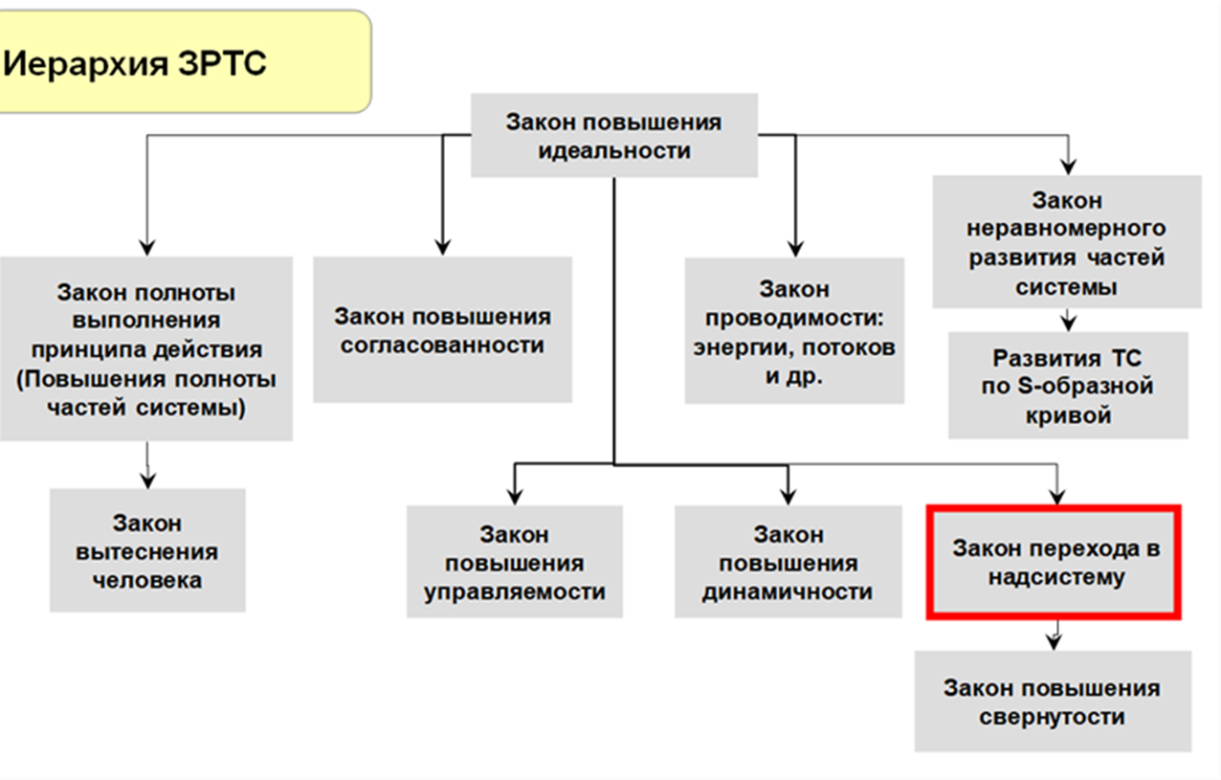
\includegraphics[width=.9\textwidth]{oE4yUs.png}
\end{center}
\begin{quote}
  Dies sind von oben nach unten und von links nach rechts
  \begin{itemize}
  \item Das Gesetz der Erhöhung der Idealität.
  \item Das Gesetz der Vollständigkeit des Aktionsprinzips (Erhöhung der
    Voll\-stän\-dig\-keit der Teile des Systems)
  \item Das Gesetz der Erhöhung der Abstimmung.
  \item Das Gesetz der Durchlässigkeit (von Energie, Flüssen usw.)
  \item Das Gesetz der ungleichmäßigen Entwicklung der Teile des Systems
  \item Die Entwicklung des technischen Systems längs einer S-Kurve
  \item Das Gesetz der Verdrängung des Menschen
  \item Das Gesetz der Erhöhung der Steuerbarkeit
  \item Das Gesetz der Erhöhung der Dynamität
  \item Das Gesetz des Übergangs zum Obersystem
  \item Das Gesetz der Erhöhung der Interdependenzen
  \end{itemize}
\end{quote}
Analysieren Sie die Entwicklungsstadien des Kinos mithilfe der
Entwicklungsgesetze technischer Systeme. Was lässt sich unter Berücksichtigung
der von Ihnen identifizierten Trends für die weitere Entwicklung des Kinos
vorhersagen?

\subsection*{Nomination „Forschung“}
\kinogenres
\subsection*{Nomination „TRIZ Videos“}
\kinotools

\video


\end{document}
